\chapter{Implementation details}

The meta-model generation mechanism is implemented as an annotation processor, hereafter referred to as "domain-model processor".

\begin{figure}[H]\centering
    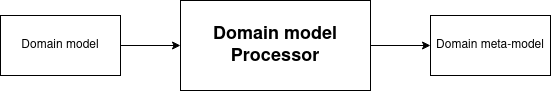
\includegraphics[scale=0.65]{images/implement1.drawio.png}
    \caption[Input and output of the annotation processor]{Annotation processor accepts a processing environment on input and produces generated sources on output}\label{fig:implement1}
\end{figure}

The annotation processor is initialized with a processing environment, by the compiler.
The processing environment provides an AST that was obtained by parsing source files.
In the incremental compilation environments, the processor benefits from the fact that it is possible to access the AST of a source file that was not necessarily a part of the compiler’s input.

\section{Entity graph}
A convenient and intuitive model for entities and their properties is a graph.
The structure of an entity can be represented as a directed graph where each node is a type, with the \textit{source} being the type of the entity itself.
A domain graph must include all entity nodes, thus it may have multiple sources.
An arc $(x, y)$ can be read as "Entity $x$ has a property of type $y$". 

\n

Figure \ref{fig:entity-graph} depicts a graph for entity \texttt{Person}, \texttt{User} and \texttt{Vehicle}.
The labels attached to arcs are the corresponding names of those properties.
All nodes are labeled with their type’s name.
The ones filled with blue are entity types, while those filled with white, which are always sinks, are non-entity types.
An entity graph might contain a cycle.
For example, the above graph contains one cycle $(User, User)$ at the \texttt{basedOnUser} property.

\begin{figure}[H]\centering
    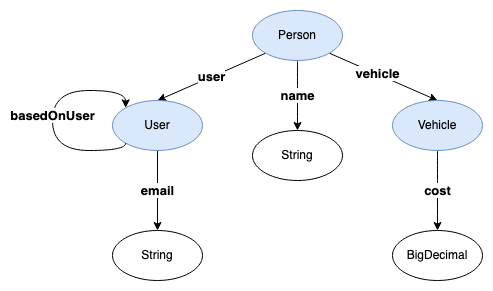
\includegraphics[scale=0.65]{images/entity-graph.drawio.png}
    \caption{\texttt{Person} entity graph}\label{fig:entity-graph}
\end{figure}

\section{Meta-model generation algorithm}
At the highest level the meta-model generation mechanism functions according to the following rules:
\begin{itemize}
    \item For each class annotated with \texttt{@MapEntityTo} or \texttt{@DomainEntity} there will be a meta-model generated that captures all of its properties, that is, all fields annotated with \texttt{@IsProperty}.
    \item A meta-models collection class will be generated. This class is a container storing an instance of every active meta-model in a static field. In other words, it contains an entity graph for each domain entity.
    \item Whenever a domain entity is modified, the whole entity graph is considered for regeneration. That is, each node representing a domain entity will have its metamodel regenerated. The renaming and deletion of an entity is also covered.
    \item If an entity should no longer be metamodeled, that is, it is either no longer annotated with the above mentioned annotations or deleted, then its meta-model is regenerated into an inactive one. Its entity graph is removed from the meta-models collection class.
\end{itemize}


\begin{figure}[H]\centering
    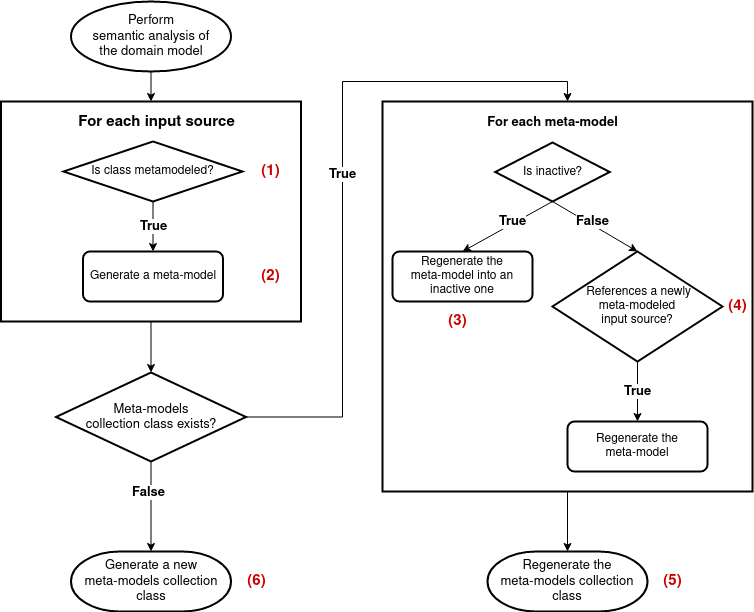
\includegraphics[scale=0.55]{images/algorithm.drawio.png}
    \caption{A high-level view of the meta-model generation algorithm}\label{fig:algorithm}
\end{figure}

\begin{enumerate}[label={\textbf{(\arabic*)}}]
    \item A class is considered to be metamodeled if it’s annotated with \texttt{@MapEntityTo} or \texttt{@DomainEntity}.
    \item This step is illustrated in detail by \ref{fig:meta-model_algorithm}. See \textbf{(2)*}
    \item A meta-model is considered to be inactive if its underlying entity no longer qualifies for being metamodeled. An inactive meta-model is structured in such a way that it effectively becomes "useless". To achieve this in Java we generate an abstract empty class (with no members). The fact that the class is abstract means that it cannot be instantiated. The reasoning behind this choice was to overcome the limitations of an inability to support deletion of meta-models.
    \item In case an entity becomes metamodeled, it is necessary to connect its meta-model to any existing ones, the underlying entities of which are adjacent in the entity graph. In other words, this step is responsible for connecting the entity graphs. This step is discussed in more detail below (\ref{fig:meta-model_graph}). See \textbf{(4)*}.
    \item The meta-models collection class is regenerated by removing fields with inactive meta-models and adding fields for newly generated meta-models if needed.
    \item This step is equivalent to \textbf{(5)}, except that there are no inactive meta-models, since the collection class does not yet exist.
\end{enumerate}

\begin{enumerate}[label={\textbf{(\arabic*)*}}]
\setcounter{enumi}{1}
    \item \;
        \begin{figure}[H]\centering
            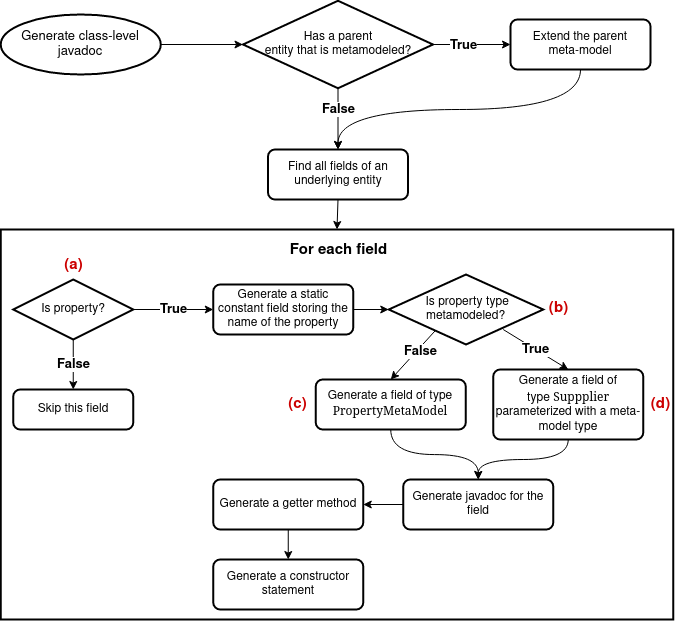
\includegraphics[scale=0.55]{images/meta-model-algorithm.drawio.png}
            \caption{The procedure of generating a meta-model}\label{fig:meta-model_algorithm}
        \end{figure}

        \begin{enumerate}[label={\textbf{(\alph*)}}]
            \item Each field annotated with \texttt{@IsProperty} is considered to be a property of an entity.
            \item See \textbf{(1)} above.
            \item \texttt{PropertyMetaModel} class is used to represent any property that is a sink in the entity graph.
            \item \texttt{Supplier<T>} is a parameterized type used to represent any node in a graph that is not a sink, where \texttt{T} is a meta-model class. This particular type is used in order to achieve lazy computation of an entity node value, since an entity graph may contain a cycle.
        \end{enumerate}

    \addtocounter{enumi}{1}
    \item Consider a situation where \texttt{Person} and \texttt{User} entities are metamodeled, while the \texttt{Vehicle} entity is not. Then the following meta-model graph exists:


        \begin{figure}[H]\centering
            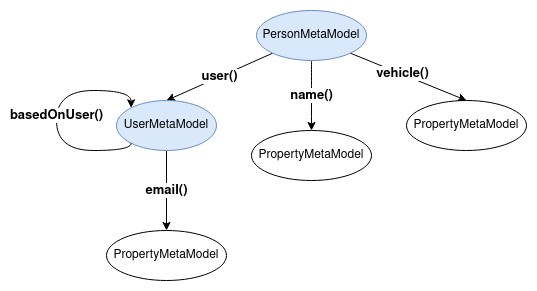
\includegraphics[scale=0.65]{images/meta-model-graph.drawio.png}
            \caption{A meta-model graph for entity \texttt{Person,} where \texttt{User} is metamodeled, but \texttt{Vehicle} is not}\label{fig:meta-model_graph}
        \end{figure}

    Then, if the entity \texttt{Vehicle} becomes metamodeled, the arc $(PersonMetaModel, PropertyMetaModel)$ labeled \texttt{vehicle()} should be replaced by an arc $(PersonMetaModel, VehicleMetaModel)$, effectively connecting both graphs.


        \begin{figure}[H]\centering
            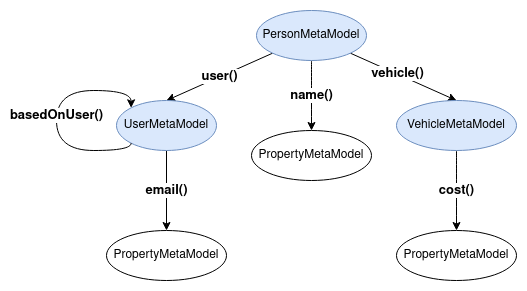
\includegraphics[scale=0.65]{images/meta-model-graph1.drawio.png}
            \caption{A meta-model graph for entity \texttt{Person} after \texttt{Vehicle} was metamodeled}\label{fig:meta-model_graph1}
        \end{figure}

    This can be achieved only by traversing each entity graph in order to find the appropriate adjacent entity nodes ($(Person, Vehicle)$ in the example above).
\end{enumerate}

\section{Meta-model structure}

The following UML class diagram illustrates the structure of the generated meta-models for entities from the example in \ref{fig:entity-graph}.

\begin{figure}[H]\centering
    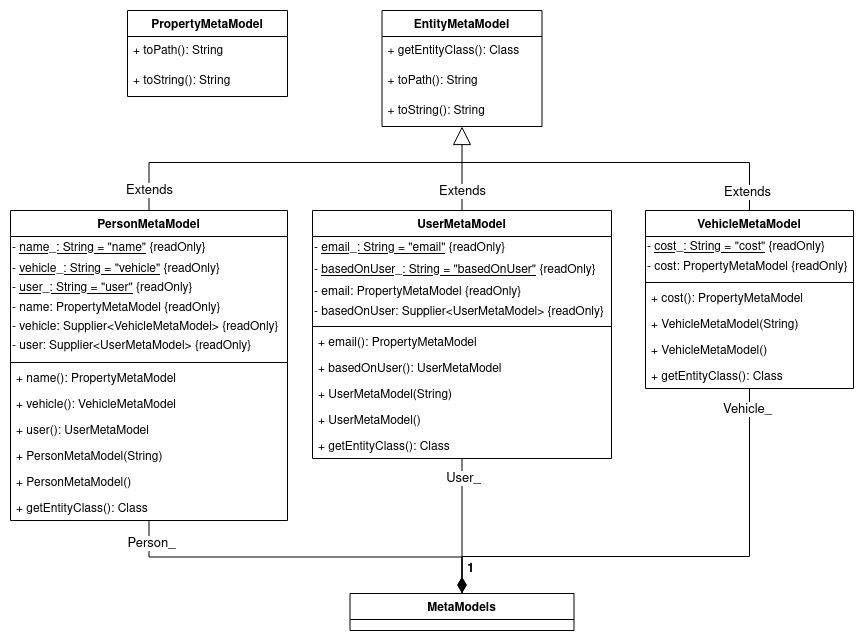
\includegraphics[scale=0.55]{images/meta-model-uml.drawio.png}
    \caption[UML class diagram for generated meta-models]{UML class diagram describing the generated meta-models for the domain illustrated in Figure \ref{fig:entity-graph}}\label{fig:meta-model_uml}
\end{figure}

The actual \texttt{String} value representing the property dot-notation is accessed by calling the \texttt{toPath()} method (or the equivalent \texttt{toString()}). 
A meta-model also implements a \texttt{getEntityClass()} method that can be used to obtain the class of its underlying entity.
Fields of the meta-models collection class (\texttt{MetaModels}) are named by appending the underscore to the name of the underlying entity in order to avoid conflicts that might be caused by static imports in Java (\texttt{Person} as type and \texttt{Person} as statically imported field).
Methods of a meta-model that are used to traverse the entity graph contain additional information about the modeled properties in the form of javadoc as illustrated below:

\n

\begin{listing}[H]
    \begin{minted}{java}
    @IsProperty
    @Title("Name", desc = "The name of this person")
    @MaxLength(255)
    private String name;
    \end{minted}
    \caption{An arbitrary non-entity type property (a sink node in the graph)}
    \label{lst:prop-sink}
\end{listing}

\begin{listing}[H]
    \begin{minted}{java}
    /**
    * Title: Name
    * Description: The name of this person
    * Type: {@link String}
    * {@literal @}{@link IsProperty}
    * {@literal @}{@link MaxLength}(value = 255)
    */
    public PropertyMetaModel name() {
        return this.name;
        }
    \end{minted}
    \caption{A property metamodeled after \ref{lst:prop-sink}}
    \label{lst:meta-prop-sink}
\end{listing}

\begin{listing}[H]
    \begin{minted}{java}
    @IsProperty
    @Title("User", desc = "User associated with this person")
    private User user;
    \end{minted}
    \caption{An arbitrary entity-type property}
    \label{lst:prop-entity}
\end{listing}

\begin{listing}[H]
    \begin{minted}{java}
    /**
     * Title: User
     * Description: User associated with this person
     * Type: {@link User}
     * Meta-model: {@link UserMetaModel}
     * {@literal @}{@link IsProperty}
     */
    public UserMetaModel user() {
        return this.user.get();
    }
    \end{minted}
    \caption{A property metamodeled after \ref{lst:prop-entity}}
    \label{lst:meta-prop-entity}
\end{listing}


\section{Usage example}
\begin{listing}[H]
    \begin{minted}[linenos]{java}
    public class PersonFetcher {
        static final PersonMetaModel person = MetaModels.Person;
            
        // a fetch model used to fetch data from a database
        static final Fetch<Person> FETCH = fetch(Person.class).with(
                // sink node
                person.name(),                   // "name"

                // entity node
                person.user(),                   // "user"
                person.user().basedOnUser(),     // "user.basedOnUser"
                person.vehicle(),                // "vehicle"
                person.vehicle().cost(),         // "vehicle.cost"

                // source node
                person                           // "this"
                );
    }
    \end{minted}
    \caption{Using the meta-model for entity \texttt{Person} to traverse its graph}
    \label{lst:person_meta-model_usage}
\end{listing}

Suppose that the conceptual schema has changed, resulting in the \texttt{Vehicle} entity no longer having the property \texttt{cost}. Then, the following compilation error would occur at line 13:
\begin{minted}[escapeinside=||]{java}
    // error: The method cost() is undefined for the type VehicleMetaModel
    person.vehicle().|\textcolor{red}{\uwave{\textcolor{black}{cost()}}}|,
\end{minted}

\n

The true power of a meta-model is manifested in combination with code auto-completion:

\begin{figure}[H]\centering
    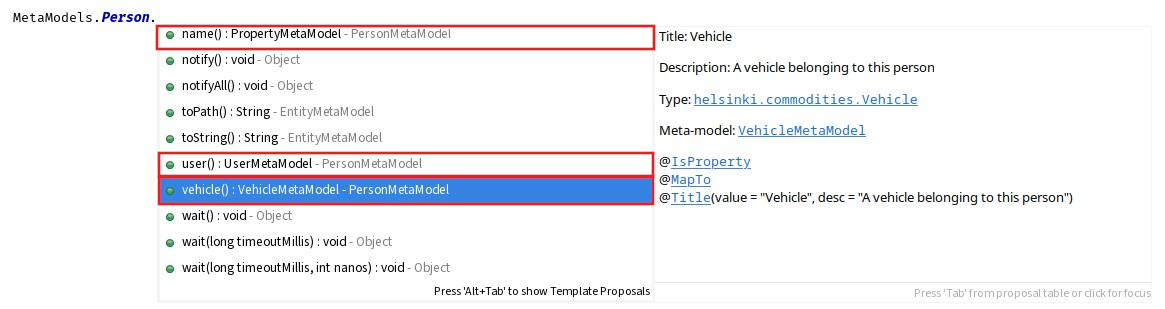
\includegraphics[scale=0.5]{images/eclipse-hl.jpg}
    \caption[Traversing the entity graph with the help of Eclipse IDE code auto-completion feature]{Traversing the entity graph with the help of Eclipse IDE code auto-completion feature
    \\
    \textit{Note}: Property-methods are highlighted}\label{fig:meta-model_uml}
\end{figure}


